\subsection{Angles and Sectors of Circles}
Mathematicians tend to deal mostly with \dfont{radians} and we 
will see later that some formulas are more elegant when using 
radians (rather than degrees). The relationship between degrees 
and radians is:
$$\pi~\mbox{rad}=180^\circ.$$
Using this formula, some common angles can be derived:
$$\begin{array}{|c|c|c|c|c|c|c|c|c|c|c|c|}
\hline
~ & ~ & ~ & ~ & ~ & ~ & ~ & ~ & ~ & ~ & ~ & ~ \\
\mbox{Degrees} & 0^\circ & 30^\circ & 45^\circ & 60^\circ & 90^\circ & 120^\circ & 135^\circ & 150^\circ & 180^\circ & 270^\circ & 360^\circ \\
~ & ~ & ~ & ~ & ~ & ~ & ~ & ~ & ~ & ~ & ~ & ~ \\
\hline
~ & ~ & ~ & ~ & ~ & ~ & ~ & ~ & ~ & ~ & ~ & ~ \\
\mbox{Radians} & 0 & \ds{\frac{\pi}{6}} & \ds{\frac{\pi}{4}} & \ds{\frac{\pi}{3}} & \ds{\frac{\pi}{2}} & \ds{\frac{2\pi}{3}} & \ds{\frac{3\pi}{4}} & \ds{\frac{5\pi}{6}} & \ds{\pi} & \ds{\frac{3\pi}{2}} & 2\pi\\
~ & ~ & ~ & ~ & ~ & ~ & ~ & ~ & ~ & ~ & ~ & ~ \\
\hline
\end{array}$$

\begin{example}{Degrees to Radians}{DegreesToRadians}
To convert $45^\circ$ to radians, multiply by $\ds{\frac{\pi}{180^\circ}}$ to get $\ds{\frac{\pi}{4}}$.
\end{example}

\begin{example}{Radians to Degrees}{RadiansToDegrees}
To convert $\ds{\frac{5\pi}{6}}$ radians to degrees, multiply by $\ds{\frac{180^\circ}{\pi}}$ to get $150^\circ$.
\end{example}

From now on, unless otherwise indicated, we will \ifont{always} use radian measure.

In the diagram below is a sector of a circle with \dfont{central angle} 
$\theta$ and radius $r$ \dfont{subtending} an arc with length $s$.

$$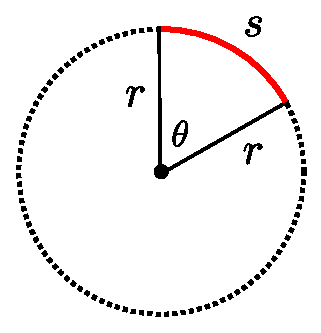
\includegraphics[width=50mm]{images/trig1}$$

When $\theta$ is measure in radians, we have the following 
formula relating $\theta$, $s$ and $r$:
$$\theta=\frac{s}{r}\mbox{\quad~or\quad}s=r\theta.$$

\begin{formulabox}[Sector Area]
The area of the sector is equal to:
$$\mbox{Sector Area}=\frac{1}{2}r^2\theta.$$
\end{formulabox}

\begin{example}{Angle Subtended by Arc}{AngleSubtendedArc}
If a circle has radius $3$ cm, then an angle of $2$ rad is subtended 
by an arc of $6$ cm ($s=r\theta=3\cdot 2=6$).
\end{example}

\begin{example}{Area of Circle}{AreaOfCircle}
If we substitute $\theta=2\pi$ (a complete revolution) into the sector 
area formula we get the area of a circle: 
$$A=\frac{1}{2}r^2(2\pi)=\pi r^2.$$
\end{example}